\documentclass[11pt,a4paper,notitlepage]{article}
\usepackage[margin = 1.5cm]{geometry}
\usepackage[utf8]{inputenc}
\usepackage{lmodern}
\usepackage[T1]{fontenc} 
\usepackage{microtype}
\usepackage{inconsolata}
\usepackage[icelandic,english]{babel}
\selectlanguage{english}
\usepackage{amsmath}
\usepackage{amsfonts}
\usepackage{mathtools}
\usepackage{amssymb}
\usepackage{amsthm}
\usepackage{enumerate}
\usepackage{multicol}
\usepackage{tasks}
\usepackage{xcolor,colortbl}
\usepackage{siunitx}
\usepackage{caption}
\usepackage{subcaption}
\usepackage{etoolbox}
\usepackage{graphicx}
\usepackage{float}
\usepackage{booktabs}
\usepackage{tikz}
\usetikzlibrary{shapes}
\usepackage{hyperref}
\usepackage{menukeys}
\renewmenumacro{\keys}{shadowedroundedkeys}
\hypersetup
{
    colorlinks=true,
    linkcolor=black,
    citecolor=black,
    filecolor=black, 
  	urlcolor=black,
}
\usepackage[all]{hypcap}
\usepackage{verbatim}
\definecolor{bluekeywords}{rgb}{0.13,0.13,1}
\definecolor{greencomments}{rgb}{0,0.5,0}
\definecolor{redstrings}{rgb}{0.9,0,0}
\definecolor{backgroundgray}{rgb}{0.95,0.95,0.95}
\usepackage{listings}
\lstset{language=Java,
showspaces=false,
numberstyle=\tiny\color{black},
backgroundcolor=\color{backgroundgray},
showtabs=false,
breaklines=true,
captionpos=b,
numbers=left,
showstringspaces=false,
breakatwhitespace=true,
escapeinside={(*@}{@*)},
commentstyle=\color{greencomments},
keywordstyle=\color{bluekeywords}\bfseries,
stringstyle=\color{redstrings},
basicstyle=\ttfamily\small
}

\newcommand{\B}{\mathbb{B}} % binary set
\newcommand{\N}{\mathbb{N}} % set of natural numbers
\newcommand{\Z}{\mathbb{Z}} % set of integers 
\newcommand{\Q}{\mathbb{Q}} % set of rationals
\newcommand{\R}{\mathbb{R}} % set of reals
\newcommand{\C}{\mathbb{C}} % set of complex
\newcommand{\map}[3]{#1: #2 \to #3} % 1 : 2 -> 3
\newcommand{\der}[1]{\frac{d}{d#1}} % derivative
\newcommand{\set}[1]{\left\{#1\right\}} % set, general
\newcommand{\nset}[1]{\set{1,2,\ldots,#1}} % {1,2,...,n}
\newcommand{\cata}[1]{\frac{1}{#1+1}\binom{2#1}{#1}} % catalan numbers
\renewcommand{\vector}[1]{(x_1,x_2,\ldots,x_{#1})} % x-vector, len n
\newcommand{\avector}[2]{(#1_1,#1_2,\ldots,#1_{#2})} % ?-vector, len n
\newcommand{\vvec}[1]{\begin{pmatrix}#1\end{pmatrix}}
\newcommand{\mc}[1]{\mathcal{#1}}
\newcommand{\ttt}[1]{\texttt{#1}}
\newcommand{\ilim}[1]{\lim_{#1\to\infty}}
\newcommand{\bpar}[1]{\left(#1\right)}
\newcommand{\floor}[1]{\left\lfloor #1 \right\rfloor}
\theoremstyle{definition}
\newtheorem{axiom}{Axiom}[section]
\newtheorem{proposition}{Proposition}[section]
\newtheorem{corollary}{Corollary}[section]
\newtheorem{lemma}{Lemma}[section]
\newtheorem{example}{Example}[section]
\newtheorem*{remark}{Remark}
\newtheorem*{note}{Note}
\newtheorem{definition}{Definition}[section]
\renewcommand\lstlistlistingname{List of Listings}

\newcommand{\maketitlepage}
{
  \begin{titlepage}
    \begin{center}
      \ \\[2.5cm]
      
\includegraphics[width=0.65\textwidth]{rulogo.png}\\[2.5cm]
      \textsc{\Huge Artificial Intelligence}\\[.5cm]
      \textsc{\huge Minesweeper}\\[.5cm]
      \textsc{\LARGE Final Project}\\[1.2cm]
      \textsc{\Large \today}\\[4cm]
      \textsc{\huge Jón Steinn Elíasson}\\[.3cm]      
      \text{jonse07@ru.is}
    \end{center}
    \vfill
  \end{titlepage}
}

\newcommand{\maketocpage}
{
  \tableofcontents
  \listoftables
  \listoffigures
  \lstlistoflistings
  \vfill
  \clearpage
}

\begin{document}
\maketitlepage
\maketocpage

\section{Introduction}
Minesweeper is a single player logic puzzle game popularized by windows but originally from the 1960s. \cite{wiki} The game is played on a grid of cells where some cells contain a bomb. Originally all cells are closed and the goal is to open all that do not contain a bomb. 

\begin{definition}
A \emph{Minesweeper board} $\mathcal{B} = (B,b)$ is a pair of $n \times k$ grid of cells, \begin{align*}
B = \set{1,2,\ldots,n} \times \set{1,2,\ldots,k} \subset \N^2
\end{align*}
where $n$ and $k$ are the number of cells horizontally and vertically respectively and a function $b : B \to \set{0,1}$ that maps each cell to the number of bombs it contains.
\end{definition}
\begin{example}
The Minesweeper board in figure \ref{fig:msb} shows the grid and the function $b$ of each cell. It is defined by $\mathcal{B} = (B,b)$ where
\begin{align*}
B = \set{(1,1),(2,1),(3,1),(1,2),(2,2),(3,2)}
\end{align*}
and
\begin{align*}
b(x,y) = 
\begin{cases} 
1 \mbox{ if } (x,y) \in \set{(1,2),(3,2)}\\
0 \mbox{ otherwise}
\end{cases}
\end{align*}
\begin{figure}[H]
\begin{center}
\begin{tikzpicture}
\draw (0,0) grid (3,2);
\draw (0.5,0.5) node {$1$};
\draw (2.5,0.5) node {$1$};
\draw (0.5,1.5) node {$0$};
\draw (1.5,0.5) node {$0$};
\draw (1.5,1.5) node {$0$};
\draw (2.5,1.5) node {$0$};
\draw (0,0.5) node[left] {$2$};
\draw (0,1.5) node[left] {$1$};
\draw (.5,0) node[below] {$1$};
\draw (1.5,0) node[below] {$2$};
\draw (2.5,0) node[below] {$3$};
\end{tikzpicture}
\end{center}
\caption{Minesweeper board example}
\label{fig:msb}
\end{figure}
\end{example}

\begin{definition}
For a cell $(x,y) \in B$ in a Minesweeper board $\mathcal{B} = (B,b)$, the set of surrounding cells,
\begin{align*}
\text{adj}(x,y) = \set{(x+i,x+j) : (i \neq 0 \vee j \neq 0) \wedge i,j \in \set{-1,0,1} \wedge (x+i,x+j) \in B},
\end{align*}
is called the \emph{adjacent cells}.
\end{definition}
\begin{example}
Table \ref{table:ac} shows the adjacent cells for all cells in the Minesweeper board in figure \ref{fig:msb}.
\begin{table}[H]
\begin{center}
\begin{tabular}{c|l}
Cell & Adjacent cells \\
\hline
$(1,1)$ & $\set{(1,2),(2,1),(2,2)}$ \\
$(2,1)$ & $\set{(1,1),(3,1),(1,2),(2,2),(3,2)}$ \\
$(3,1)$ & $\set{(2,1),(2,2),(3,2)}$ \\
$(1,2)$ & $\set{(1,1),(2,1),(2,2)}$ \\
$(2,2)$ & $\set{(1,1),(2,1),(3,1),(1,2),(3,2)}$ \\
$(3,2)$ & $\set{(2,1),(3,1),(2,2)}$
\end{tabular}
\end{center}
\caption{Adjacent cells}
\label{table:ac}
\end{table}
\end{example}

\begin{definition}
Given a Minesweeper board $\mathcal{B} = (B,b)$, let $E = \set{(x, y) : (x,y) \in B \wedge b(x,y) = 0}$, that is the set of cells with no bomb. For any cell $(x,y) \in E$, we say that the \emph{adjacency number} of $(x,y)$ is $\sum_{c \in \text{adj}(x,y)}b(c)$.
\end{definition}

\begin{example}
Table \ref{table:an} shows all adjacency numbers for the Minesweeper board from figure \ref{fig:msb}.
\begin{table}[H]
\begin{center}
\begin{tabular}{c|c}
Cell & Adjacency number \\
\hline
$(1,1)$ & $1$ \\
$(2,1)$ & $2$ \\
$(3,1)$ & $1$ \\
$(2,2)$ & $2$
\end{tabular}
\end{center}
\caption{Adjacency numbers}
\label{table:an}
\end{table}
\end{example}

When playing the game, if a cell does not contain a bomb it shows the adjacency number when opened. Figure \ref{fig:brdexamp} shows an example of a board where all cells have been opened, marking bombs with $X$. The game is lost by opening a cell with a bomb. 
\begin{figure}[H]
\begin{center}
\begin{tikzpicture}
\draw (0,0) grid (4,4);
\draw (0.5, 3.5) node {$0$};\draw (1.5, 3.5) node {$2$};\draw (2.5, 3.5) node {$X$};\draw (3.5, 3.5) node {$X$};
\draw (0.5, 2.5) node {$0$};\draw (1.5, 2.5) node {$2$};\draw (2.5, 2.5) node {$X$};\draw (3.5, 2.5) node {$3$};
\draw (0.5, 1.5) node {$1$};\draw (1.5, 1.5) node {$3$};\draw (2.5, 1.5) node {$2$};\draw (3.5, 1.5) node {$2$};
\draw (0.5, 0.5) node {$X$};\draw (1.5, 0.5) node {$2$};\draw (2.5, 0.5) node {$X$};\draw (3.5, 0.5) node {$1$};
\end{tikzpicture}
\end{center}
\caption{Complete $4 \times 4$ minesweeper board}
\label{fig:brdexamp}
\end{figure}
Although the game is simple, it can be hard to win. At some point you might have to sort to guessing, either if the player can not conclude anything from the given table or there is nothing to conclude (regardless of the player). Solving minesweeper has in fact been shown to be NP-complete \cite{npc}.\\

The main objective of this assignment is to create an agent that plays minesweeper successfully. This is a constraint satisfaction problem where the potential variables are the closed cells, their domain $\set{0,1}$ and the constraints are the requirements formed by the adjacency numbers. There is also an element of guessing when nothing can be concluded from the constraints.

\section{Motivation}
The project is chosen from a list of suggested topics. There were many interesting topics suggested but I chose Minesweeper mainly because I used to play it a lot when I was younger. Overall, I think it's a very interesting game where with simplistic rules but difficult strategies which I think is a good characteristics for a game.\\

A GUI for Minesweeper is also fairly simple and although not a requirement, I wanted to have something visual. It does add a lot to a project like this. I also thought it might be good idea to do a large programming assignment on CSP since we covered it a lot but did not have a large assignment for it.

\section{The solution}
\subsection{An overview of the approach}
The board generation is done by the GUI controller and the only information passed between it and the agent is the next move of the agent and the resulting adjacency number if not a bomb. The board is completely random and can have a bomb at the first cell the agent chooses.\\

Figure \ref{fig:aov} shows a simplified version of how the agent works. The red arrows are information being passed while the blue are state transitions, when there are no pending moves. 

\begin{figure}[H]
\begin{center}
\begin{tikzpicture}[thick,scale=0.6, every node/.style={scale=0.6,draw=black, ellipse, minimum width=25pt, text width=2cm, align=center}]
\node (a) {Actual board};
\node[right=100pt] (b) at (a) {Pending moves};
\node[below=50pt] (c) at (b) {The first move};
\node[above=50pt] (d) at (b) {Internal updating};
\node[right=100] (e) at (d) {Search for safe moves};
\node[right=100] (f) at (b) {Endgame search};
\node[right=100] (g) at (c) {Probability guess};

\draw[<-, red] (a) -- (b);
\draw[->,red] (a) -- (d);
\draw[->, red] (c) -- (b);
\draw[->, red] (e) -- (b);
\draw[->, red] (f) -- (b);
\draw[->, red] (g) -- (b);
\draw[->, red] (d) -- (b);
\draw[->,red] (f) -- (d);
\draw[->,red] (e) -- (d);

\draw[->,blue] (e) -- (f);
\draw[->,blue] (f) -- (g);
\draw[->,blue] (e) to[bend left=75] (g);
\end{tikzpicture}
\end{center}
\caption{Agent overview}
\label{fig:aov}
\end{figure}

Until a game is lost or won, the agent is asked for his next move and the resulting adjacency number sent back. The agent has a collection of pending moves which is initially contains the opening move. If any moves are pending, some move is sent to the GUI controller and removed from the pending moves.\\

The agent keeps track of his own board, from his perspective. At any time the agent receives an adjacency number or finds a bomb, he updates his internal perspective of the board and adds, removes or changes constraints. This is repeated for any bomb that he does find when updating. All safe cells he finds are added to the pending moves.\\

If the collection of pending moves becomes empty, we split the constraint into groups, disjoint of variables and search each for guarantees. Any bombs found are passed to internal updating while safe cells are added to pending moves. If no safe cells are found we check if we are in the endgame and if so add an additional constraint and try again.\\

If no safe cells have been found at this point, we resort to guessing. This is done by calculating the probability of each variable containing a bomb and picking the least likely but we also consider the unknown cells that are not considered variables.

\subsection{Board generation}
There are 4 different types of board generation, set by two boolean flags, all of whom are randomly generated. The first flag prevents bomb being surrounded, shown by the shaded cells in figure \ref{fig:nosurr}.\\

\begin{figure}[h]
\begin{center}
\begin{tikzpicture}
\fill[gray!10] (1,1) rectangle (2,2);
\fill[gray!10] (6,2) rectangle (7,3);
\draw (0,0) grid (3,3);
\draw (4,0) grid (7,3);
\draw (.5,.5) node {$X$};
\draw (1.5,.5) node {$X$};
\draw (2.5,.5) node {$X$};
\draw (.5,1.5) node {$X$};
\draw (2.5,1.5) node {$X$};
\draw (.5,2.5) node {$X$};
\draw (1.5,2.5) node {$X$};
\draw (2.5,2.5) node {$X$};
\draw (6.5,1.5) node {$X$};
\draw (5.5,1.5) node {$X$};
\draw (5.5,2.5) node {$X$};
\end{tikzpicture}
\caption{Generation with no surrounded bombs}
\label{fig:nosurr}
\end{center}
\end{figure}

The second flag recursively splits the generation into 2 or 4 parts (horizontally, vertically or both) to spread bombs more evenly. This is only done if the size of the part (or the whole board initially) is larger than a set max width/height. This is demonstrated in figure \ref{fig:recspl} where 3 bombs are on each side, horizontally. 

\begin{figure}[H]
\begin{center}
\begin{tikzpicture}[thick,scale=0.5, every node/.style={scale=0.35}]
\fill[gray!10] (0,0) rectangle (4,4);
\fill[gray!30] (4,0) rectangle (8,4);
\draw (0,0) grid (8,4);
\draw[thick] (4,0) -- (4,4);
\draw (1.5,0.5) node {$X$};
\draw (3.5,1.5) node {$X$};
\draw (2.5,3.5) node {$X$};
\draw (7.5,3.5) node {$X$};
\draw (7.5,2.5) node {$X$};
\draw (6.5,1.5) node {$X$};
\end{tikzpicture}
\caption{Generation with bomb spreading}
\label{fig:recspl}
\end{center}
\end{figure}

\subsection{GUI}
The GUI does not support changes of the generation mechanics and the final version has both flags as false so the board generated is completely random. There are 3 fixed level settings in the GUI shown in table \ref{table:lvl}, modeled after the initial Microsoft version. 
\begin{table}[H]
\begin{center}
\begin{tabular}{ccccc}
Name & Width & Height & Bombs \\
\hline
Small & 8 & 8 & 10 \\
Medium & 16 & 16 & 40 \\
Large & 24 & 24 & 99
\end{tabular}
\caption{Different levels}
\label{table:lvl}
\end{center}
\end{table}

Playing as a human is supported although mostly for fun. A screen shot of the GUI can be seen in figure \ref{fig:gui}, which is of the small level setting. The start button is enabled if you set the player as \texttt{Computer} and will play the game as the agent. The labels next to it are the bombs remaining and a timer.

\begin{figure}[H]
\begin{center}
\begin{minipage}{0.3\textwidth}
\begin{figure}[H]
\begin{center}
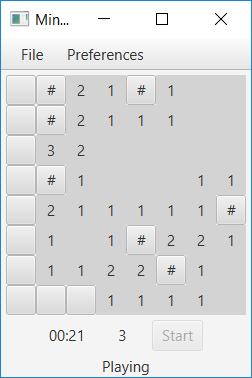
\includegraphics[scale=0.8]{GUI.png}
\end{center}
%\caption{The GUI}
%\label{fig:gui}
\end{figure}
\end{minipage}
\hspace{1cm}
\begin{minipage}{0.3\textwidth}
\begin{table}[H]
\begin{center}
\begin{tabular}{cl}
%Button & Functionality \\
%\hline
\keys{Esc} & quit \\
\keys{F1} & new game \\
\keys{F2} & start (computer only) \\
\keys{1} & small board \\
\keys{2} & medium board \\
\keys{3} & large board
\end{tabular}
\end{center}
%\caption{Keyboard shortcuts}
%\label{table:sc}
\end{table}
\end{minipage}
\end{center}
\caption{The GUI}
\label{fig:gui}
\end{figure}

\subsection{Opening}%TODO rewrite
The opening move is a random non-edge cell. The reason for avoiding edges is that any adjacency number other than 0 will result in worse probabilities in adjacent cells than another random guess outside them while a adjacency number of 1 in a non-edge cell will result in the adjacent cells being more likely than a random guess outside them.
\begin{figure}[H]
\begin{center}
\begin{tikzpicture}
\fill[green!20] (0,0) rectangle (4,4);
\fill[red!20] (0,1.5) rectangle (1,3);
\fill[white] (0,2) rectangle (0.5,2.5);
\draw[step=0.5] (0,0) grid (4,4);
\draw (0.25,2.25) node {$1$};
\end{tikzpicture}
\hspace{1cm}
\begin{tikzpicture}
\fill[green!20] (0,0) rectangle (4,4);
\fill[red!20] (1.5,2) rectangle (3,3.5);
\fill[white] (2,2.5) rectangle (2.5,3);
\draw (2.25,2.75) node {$1$};
\draw[step=0.5] (0,0) grid (4,4);
\end{tikzpicture}
\end{center}
\caption{Opening move}
\label{fig:open}
\end{figure}
In figure \ref{fig:open} we can see two scenarios, both a $8\times 8$ board with 10 bombs, one where the opening cell is on an edge and one where it isn't. In the first case, we have 
\begin{align*}
P(\text{red}) = 1/5 = 0.2 \text{ and } P(\text{green}) = 9 / (8 \cdot 8 - 6) = 9/58 \approx 0.155,
\end{align*}
so we would guess at random in the green ones in this case. In the latter, we have
\begin{align*}
P(\text{red}) = 1/8 = 0.125 \text{ and } P(\text{green}) = 9/ (8 \cdot 8 - 9) = 9/55 \approx 0.164, 
\end{align*}
and we would choose a red cell at random. Finding an adjacency number of 0 at start would be best but if we get an adjacency number of 1, we prefer to do that outside the edges since that produces the least likely cells to contain bombs. Any other adjacency number in the opening move results in guesses in 'the green cells', regardless of being on an edge or not.\\

\subsection{Data structures}
The key data structure is the one that keeps track of constraints. It is a map from the position of the adjacency number to the pair of updated adjacency number and unknown adjacent cells. It is updated dynamically so no unnecessary constraint are kept (except for possible duplicates which are filtered elsewhere) and each is updated when new information is discovered. The agent also stores all his findings about the board in a 2D array.\\

Another important data structure is the constraint groups. It is a map from a set of constraints to their variables. The constraints do keep their variables internally but the reason for having them as values in a map, is ease of use for the constraint framework. When created, it starts with an empty set and goes through all the constraints and if none of the variables belong to any of pre-existing groups, a new one is created. If the variables are shared with some pre-existing groups they removed from the map, merged into a new set into which the current constraint is added which is then added back to the map. This makes sure that the constraint groups are completely independent.\\

Suppose we were making truth tables to search for satisfiability in $n$ boolean variables given some constraints, then there would be $2^n$ possible assignments. If we split those into $k$ independent groups (of equal size) we have $2^{(n/k)} + 2^{(n/k)} + \ldots + 2^{(n/k)} = k\cdot 2^{(n/k)}$ possible assignments so this reduces the problem quite a bit. Taking a numeric example, suppose $n = 15$ and $k = 3$, then $2^n =32768$ while $k \cdot 2^{(n/k)} = 96$.\\

\subsection{Internal updating}
Only unknown cells adjacent to a cell with a known adjacency number are considered variables. Any adjacency number is reduced for each known bomb we know about adjacent to it so the perspective of the board is different for the agent to how the GUI draws it. In figure \ref{fig:aper}, we see the same board with the same cells opened, where the one on the left is how the agent sees it while the right one is how the GUI shows it.
\begin{figure}[H]
\begin{center}
\begin{tikzpicture}
\draw (0,0) grid (3,3);
\draw (0.5,2.5) node {$X$};
\draw (2.5,0.5) node {$X$};
\draw (0.5,1.5) node {$1$};
\draw (1.5,1.5) node {$3$};
\end{tikzpicture}
\hspace{2cm}
\begin{tikzpicture}
\draw (0,0) grid (3,3);
\draw (0.5,2.5) node {$X$};
\draw (2.5,0.5) node {$X$};
\draw (0.5,1.5) node {$2$};
\draw (1.5,1.5) node {$5$};
\end{tikzpicture}
\end{center}
\caption{Agent's perspective compared to ours}
\label{fig:aper}
\end{figure}

\begin{definition}
An adjacency constraint is \emph{trivial} if the adjacency number is 0 or equal to the number of variables.
\end{definition}

\begin{example}
Figure \ref{fig:triv} shows both cases of trivial constraints. The adjacency number is shown on a $a/b$ format where $a$ is what the GUI would display while $b$ is what the agent would have stored internally. In the left one, we have 
\begin{align*}
\sum_{1 \leq i \leq 6}x_i = 0 \Rightarrow x_i = 0 \text{ for } i = 1,2,\ldots,6.
\end{align*}
In the right one, we have
\begin{align*}
x_1 + x_2 = 2 \Rightarrow x_1 = x_2 = 1.
\end{align*}
\begin{figure}[H]
\begin{center}
\begin{tikzpicture}
\draw (0,0) grid (3,3);
\draw (0.5,0.5) node {$X$};
\draw (2.5,1.5) node {$X$};
\draw (1.5,1.5) node {$2$/$0$};
\draw (.5,2.5) node {$x_1$};
\draw (1.5,2.5) node {$x_2$};
\draw (2.5,2.5) node {$x_3$};
\draw (0.5,1.5) node {$x_4$};
\draw (1.5,0.5) node {$x_5$};
\draw (2.5,0.5) node {$x_6$};
\end{tikzpicture}
\hspace{2cm}
\begin{tikzpicture}
\draw (0,0) grid (3,3);
\draw (1.5,1.5) node {$X$};
\draw (.5,2.5) node {$3/2$};
\draw (1.5,2.5) node {$x_1$};
\draw (0.5,1.5) node {$x_2$};
\end{tikzpicture}
\end{center}
\caption{Trivial constraints}
\label{fig:triv}
\end{figure}
\end{example}

Whenever the agent receives an adjacency number, he updates internally. We remove the cell containing the adjacency number from any constraint containing it. The new adjacency number forms a new constraint if not trivial. The adjacent cells that are unknown must add up to the number we just received, subtracted by the known bombs adjacent to it.\\

If the constraint is trivial or any updated constraint become trivial, all unknown adjacent cells are either added to pending moves or known bombs (depending on which case of trivial constraint).\\

When we learn the position of a new bomb (including those learned from the trivial constraint) we also must update any constraint containing its cell. They are removed from the constraint and the adjacency number is reduced by one. If they become trivial they go through the same process as we mentioned earlier.



\subsection{Search}
If we have no pending moves, we try to conduct one logically. We begin by splitting the constraint into groups of disjoint constraints in variables. This also take cares of duplicates of any constraint by using a set.\\

\begin{figure}[H]
\begin{center}
\begin{tikzpicture}
\fill[red!20] (0,0) rectangle (1,1);
\fill[red!20] (0,2) rectangle (1,3);
\fill[green!20] (1,0) rectangle (2,1);
\fill[green!20] (1,2) rectangle (2,3);
\fill[blue!20] (2,0) rectangle (3,1);
\fill[blue!20] (2,2) rectangle (3,3);
\fill[yellow!20] (3,0) rectangle (4,1);
\fill[yellow!20] (3,2) rectangle (4,3);
\draw (0,0) grid (4,3);
\foreach \x in {1,...,4}
{
	\draw (\x - 0.5,1.5) node {$x_\x$};
	\draw (\x - 0.5,0.5) node {$2$};
	\draw (\x - 0.5,2.5) node {$2$};
}
\end{tikzpicture}
\end{center}
\caption{Duplicate constraint}
\label{fig:dc}
\end{figure}

For each constraint groups, we create a model. These constraint are propagated and stored. Then we iterate over all variables and for each, we assume that it has a bomb. If that leads to a contradiction, we know it must be safe and add it to the pending moves. If the assumption didn't lead to a contradiction, we assume that it has no bomb and if that leads to a contradiction, we update internally. After each assumption, we remove the assumption and restore the model to the propagated state from the constructor.\\

The method of checking whether anything can be concluded about a cell is shown in listing \ref{lst:choco}. The conversion from our constraint group to a Choco model has been removed for simplification and replaced by a comment.

\begin{lstlisting}[caption={Searching with Choco}, label={lst:choco}]
private Model model;
private Map<Position, IntVar> varMap;
public MSModel(Set<ConstraintInfo> constraints, Set<Position> variables) {
  /* Convert our data structures to a Choco model and create a map between the two */
  this.model.getSolver().propagate();
}
public boolean hasBomb(Position position) {
  return containsContradiction(model.arithm(varMap.get(position), "=", 0));
}
public boolean hasNoBombs(Position position) {
  return containsContradiction(model.arithm(varMap.get(position), "=", 1));
}
private boolean containsContradiction(Constraint assumption) {
  model.getEnvironment().worldPush();
  model.post(assumption);
  Solution sol = model.getSolver().findSolution();
  model.getEnvironment().worldPop(); 
  model.unpost(assumption);
  model.getSolver().hardReset();
  return sol == null;
}
\end{lstlisting}

As an example, suppose we have the following constraint group (the variables are indexed by their position where $(1,1)$ is the upper left corner),
\begin{align*}
\set{x_{(1,1)} + x_{(2,1)} = 1, x_{(1,1)}+x_{(2,1)}+x_{(3,1)} = 2},
\end{align*}
seen in figure \ref{fig:csp}. Note that the figure is from the agent's perspective.
\begin{figure}[H]
\begin{center}
\begin{tikzpicture}
\draw (0,0) grid (3,2);
\draw (.5,.5) node {$1$};
\draw (1.5,.5) node {$2$};
\draw (2.5,.5) node {$X$};
\end{tikzpicture}
\end{center}
\caption{Constraint example}
\label{fig:csp}
\end{figure}
Assuming $x_{(1,1)} = 1$ or $x_{(1,1)} = 0$, then $x_{(2,1)} = 0 \wedge x_{(3,1)}=1$ and $x_{(2,1)}=1 \wedge x_{(3,1)}=1$ satisfy the constraint respectively and we don't know if $x_{(1,1)}$ is 0 or 1. Now suppose that $x_{(3,1)} = 0$, then both $x_{(1,1)} = x_{(2,1)} = 1$ to satisfy the latter constraint which leads to a contradiction in the first so $x_{(3,1)}$ must contain a bomb.

\subsection{Guessing}
If we do not find any moves we must resort to guessing. We can still do better than random. Suppose we have the constraints shown in figure \ref{fig:prob}.
\begin{figure}[H]
\begin{center}
\begin{tikzpicture}
\draw (0,0) grid (3,4);
\draw (1.5,1.5) node {$1$};
\draw (1.5,2.5) node {$2$};
\draw (0.5,3.5) node {\tiny $X_{(1,1)}$};
\draw (1.5,3.5) node {\tiny $X_{(2,1)}$};
\draw (2.5,3.5) node {\tiny $X_{(3,1)}$};
\draw (0.5,0.5) node {\tiny $X_{(1,4)}$};
\draw (1.5,0.5) node {\tiny $X_{(2,4)}$};
\draw (2.5,0.5) node {\tiny $X_{(3,4)}$};
\draw (0.5,1.5) node {\tiny $X_{(1,3)}$};
\draw (2.5,1.5) node {\tiny $X_{(3,3)}$};
\draw (0.5,2.5) node {\tiny $X_{(1,2)}$};
\draw (2.5,2.5) node {\tiny $X_{(3,2)}$};
\end{tikzpicture}
\end{center}
\caption{Board probabilities}
\label{fig:prob}
\end{figure}
If there are 2 bombs in the top row, there must be exactly 1 bomb in the bottom row, a total of $\binom{3}{2} \cdot \binom{3}{1}$ possibilities. If there is 1 bomb in the top row, there must be no bombs in the bottom row and one bomb in the middle rows, a total of $\binom{3}{1} \cdot \binom{4}{1}$ possibilities. There can't be more than 2 in the top row or less than 1 so we have covered all possibilities. The total number of possible solutions is therefore
\begin{align*}
\binom{3}{2} \cdot \binom{3}{1} + \binom{3}{1} \cdot \binom{4}{1} = 3 \cdot 3 + 3 \cdot 4 = 9 + 12  = 21.
\end{align*}
How many times did each variable have a bomb? For the variables in the bottom row, they have a bomb one time for each of the $\binom{3}{2}$ cases of the top row having two. The middle row variables have a bomb one time for each of the $\binom{3}{1}$ cases of the top row containing 1. All of these variables therefore contain a bomb 3 times in total. The top row variables contain a bomb 2 out of 3 times for each variable in the bottom row, a total of 6 and one time for each of the middle row variables, a total of 4, yielding a grand total of 10. Now we can compute the probability for all variables,
\begin{align*}
10 / 21 \approx 0.476190476 \text{ and } 3/21 \approx 0.142857143
\end{align*}
for the top row variables and everything else, respectively. As we can see, we are much better off choosing from a row, other than the top one.\\

The constraint framework provides us with the means to get all solutions to a constraint group so we can just count the occurrences of each variable being a bomb in a given set of solution and divide it with the number of solutions. We do that and store in a probability map.\\

We do however need to take into account those unknown cells that aren't considered variables. They can have a better chance of not containing a bomb. We do that by taking the sum of the minimum number of bombs in each solution, add that to the number of bombs we know of and subtract from the initial number of bombs. This is then divided by the number of unknown cells that are not variables which gives us the worst case probability of choosing outside the variables (since we took the minimum amount of bombs in each solution). If this probability is lower than the lowest one in the map, we choose at random from the non-variables. Otherwise we pick the one in the map with the lowest probability of containing a bomb. If many exists, we pick one at random.

\subsection{End game}
A situation can arise where you can use the number of bombs remaining to conduct information about a cell. These are rare but they do happen. The constraint for that is, that the sum of all unknown cells is equal to the remaining bombs. If we would apply this at start, we would include all the cells and wouldn't split any of the constraint groups, which would have a major impact on our search.\\

This constraint can be added in the later stage of the game when the remaining cells positions are not that many. We do so at the point of 15 unknown cells left but we do not use it unless we don't find any by our normal method. If we change to end game mode for the agent, it checks between searching with constraint groups and guessing, and if something is found, we can avoid guessing.

\section{Results}
\subsection{Statistics}
No goal in terms of time was set but his solver works really fast. Any playable level available in the GUI plays instantly. Playing 3000 games, 1000 of each size, takes about 5-6 seconds. Playing 100 games on a $50 \times 50$ board with 400 bombs takes about 2.5 seconds. A single $150 \times 150$ game with $3800$ takes about 2.5 seconds to win. Timing of wins for various levels is shown in table \ref{table:time}.

\begin{table}[H]
\begin{center}
\begin{tabular}{|l|l|l|l|l|}
\hline
Width & Height & Cells & Bombs & Time (s) \\
\hline
8 & 8 & 64 & 10 & 0 \\
\hline
16 & 16 & 256 & 40 & 0 \\
\hline
24 & 24 & 576 & 99 & 0 \\
\hline
50 & 50 & 2500 & 500 & 0 \\
\hline
150 & 150 & 22500 & 3800 & 2.5 \\
\hline
500 & 500 & 250000 & 40000 & 336 \\
\hline
\end{tabular}
\end{center}
\caption{Timing of a winning play}
\label{table:time}
\end{table}

A goal of a $50\%$ win ratio was set but with no regards to which size. The following tables include statistics for 1000 games of each level, available in the GUI, and one custom game only playable in tests.

\begin{table}[H]
\begin{center}
\begin{tabular}{l|l}
Games played &  1000 \\
\hline
Games won &  846 \\
\hline
Games lost &  154 \\
\hline
Games lost on first move & 87 \\
\hline
Win ratio & 84.6\% \\
\hline
Win ratio excluding first move losses & 92.66\% \\
\end{tabular}
\end{center}
\caption{Statistics for the small map}
\label{table:sstat}
\end{table}

\begin{table}[H]
\begin{center}
\begin{tabular}{l|l}
Games played & 1000 \\
\hline
Games won & 546 \\
\hline
Games lost & 454 \\
\hline
Games lost on first move & 149 \\
\hline
Win ratio & 54.6\% \\
\hline
Win ratio excluding first move losses & 64.16\% \\
\end{tabular}
\end{center}
\caption{Statistics for the medium map}
\label{table:mstat}
\end{table}
\begin{table}[H]
\begin{center}
\begin{tabular}{l|l}
Games played & 1000 \\
\hline
Games won & 430 \\
\hline
Games lost & 570 \\
\hline
Games lost on first move & 188 \\
\hline
Win ratio & 43\% \\
\hline
Win ratio excluding first move losses & 52.96\% \\
\end{tabular}
\end{center}
\caption{Statistics for the large map}
\label{table:lstat}
\end{table}
\begin{table}[H]
\begin{center}
\begin{tabular}{l|l}
Games played & 100 \\
\hline
Games won & 41 \\
\hline
Games lost & 59 \\
\hline
Games lost on first move & 19 \\
\hline
Win ratio & 41\% \\
\hline
Win ratio excluding first move losses & 50.61\% \\
\end{tabular}
\end{center}
\caption{Statistics for a $50 \times 50$ map with 400 bombs}
\label{table:cstat}
\end{table}

From the simulations in tables \ref{table:sstat}, \ref{table:mstat} and \ref{table:lstat}, the total number of times the end game saved us from guessing was also counted.

\begin{table}[H]
\begin{center}
\begin{tabular}{c|c|c}
Small & Medium & Large \\
\hline
0 & 18 & 23
\end{tabular}
\end{center}
\caption{End game constraint saves from guessing in 1000 games}
\label{table:egs}
\end{table}
\subsection{Comparison}
In the article \href{http://www.cs.toronto.edu/~cvs/minesweeper/minesweeper.pdf}{\emph{Minesweeper as a Constraint Satisfaction Problem}} by Chris Studholme, he lists the his win ratio in a graph. The are about $68\%$, $35\%$ and $25\%$ in ascending order of difficulty. His hardest level is different from mine so if we disregard that, my solution has about $15\%$ better win ratio in the smallest game and $19\%$ in the medium one.


\section{Future work}
\subsection{Improve probability model}
As the probability is calculated now, we just take all possible solutions and count the occurrences of each variable containing a bomb in total. A group of variables belonging to a constraint group can have different number of bombs. If we would take into account, the probability of a constraint group containing some number of bombs in total (for all possible number of bombs) and use conditional probabilities we should get better results.

\subsection{Constraint simplification}
The constraints $x_1+x_2+x_3+x_4 = 2$ and $x_1+x_2=1$ can be simplified into $x_1+x_2 = 1$ and $x_3+x_4=1$. It would improve the agent if we were to handle these simplifications when splitting the constraint groups since they could potentially split some groups further.

\subsection{Explore more constraints}
A rather fun property of minesweeper is that the sum of adjacency numbers for any board is equal to the sum of adjacency numbers in its complement, that is where the bombs and empty cells have been swapped.

\begin{figure}[H]
\begin{center}
\begin{tikzpicture}
\draw (0,0) grid (5,5);
\draw (1.5,1.5) node {$X$};
\draw (1.5,3.5) node {$X$};
\draw (4.5,2.5) node {$X$};
\draw (.5,.5) node {$X$};
\draw (2.5,1.5) node {$X$};
\draw (0.5,4.5) node {$1$};
\draw (1.5,4.5) node {$1$};
\draw (2.5,4.5) node {$1$};
\draw (3.5,4.5) node {$0$};
\draw (4.5,4.5) node {$0$};
\draw (0.5,3.5) node {$1$};
\draw (2.5,3.5) node {$1$};
\draw (3.5,3.5) node {$1$};
\draw (4.5,3.5) node {$1$};
\draw (0.5,2.5) node {$2$};
\draw (1.5,2.5) node {$3$};
\draw (2.5,2.5) node {$3$};
\draw (3.5,2.5) node {$2$};
\draw (0.5,1.5) node {$2$};
\draw (3.5,1.5) node {$2$};
\draw (4.5,1.5) node {$1$};
\draw (1.5,0.5) node {$3$};
\draw (2.5,0.5) node {$2$};
\draw (3.5,0.5) node {$1$};
\draw (4.5,0.5) node {$0$};
\end{tikzpicture}
\hspace{1cm}
\begin{tikzpicture}
\draw (0,0) grid (5,5);
\draw (0.5,4.5) node {$X$};
\draw (1.5,4.5) node {$X$};
\draw (2.5,4.5) node {$X$};
\draw (3.5,4.5) node {$X$};
\draw (4.5,4.5) node {$X$};
\draw (0.5,3.5) node {$X$};
\draw (2.5,3.5) node {$X$};
\draw (3.5,3.5) node {$X$};
\draw (4.5,3.5) node {$X$};
\draw (0.5,2.5) node {$X$};
\draw (1.5,2.5) node {$X$};
\draw (2.5,2.5) node {$X$};
\draw (3.5,2.5) node {$X$};
\draw (0.5,1.5) node {$X$};
\draw (3.5,1.5) node {$X$};
\draw (4.5,1.5) node {$X$};
\draw (1.5,0.5) node {$X$};
\draw (2.5,0.5) node {$X$};
\draw (3.5,0.5) node {$X$};
\draw (4.5,0.5) node {$X$};
\draw (1.5,1.5) node {$6$};
\draw (1.5,3.5) node {$8$};
\draw (4.5,2.5) node {$5$};
\draw (.5,.5) node {$2$};
\draw (2.5,1.5) node {$7$};
\end{tikzpicture}
\end{center}
\caption{A minesweeper theorem on complements}
\label{fig:msth}
\end{figure}

In the example in figure \ref{fig:msth}, we have $3 \cdot 0 + 9 \cdot 1 + 5 \cdot 2 + 3 \cdot 3 = 28 = 2+5+6+7+8$. It would be fun to explore if this theorem (or others) could help solve the endgame.

\section{Conclusion}
Constraint satisfaction problem are usually hard to solve and often belong to high complexity problems in theory. We can however use various methods to solve them efficiently. This project is an example of that, with minesweeper being NP-complete.\\

After many days of tireless work, I'm pretty happy with the results. All my goals have been met and I have a nice little GUI to demonstrate what has been done. I had a lot of fun working on this and it was very satisfying to see it all come together (the data structures, the constraints, the probability, the GUI, etc). I would definitely recommend this as a programming assignment in the course.

\newpage
\appendix
\section{Material used}
Table \ref{table:soft} lists everything that was used in the project.
\begin{table}[H]
\begin{center}
\begin{tabular}{l|l}
Software & Usage \\
\hline
Java & Programming language \\
JavaFX & GUI \\
IntelliJ & IDE \\
JUnit4 & Testing \\
\href{http://www.choco-solver.org/}{Choco solver} & Constraint programming \\
GitHub & Source control \\
\LaTeX{} & Report, slides \\
Overleaf & Report, slides \\
\href{http://www.minesweeper.info/wiki/Strategy}{Minesweeper strategy} & Test cases \\
\href{http://www.cs.toronto.edu/~cvs/minesweeper/minesweeper.pdf}{Minesweeper as a CSP} & Research \\
\href{http://minesweeperonline.com/}{Minesweeper Online} & Play until GUI was working
\end{tabular}
\end{center}
\caption{Material used}
\label{table:soft}
\end{table}

\section{Testing}
The code is thoroughly tested, with almost 100\% coverage without the GUI which is not tested. The missing part from the \texttt{MSAgent} is a \texttt{try}-\texttt{catch} block for a Choco contradiction expectation that will never be thrown.
\begin{figure}[H]
\begin{center}
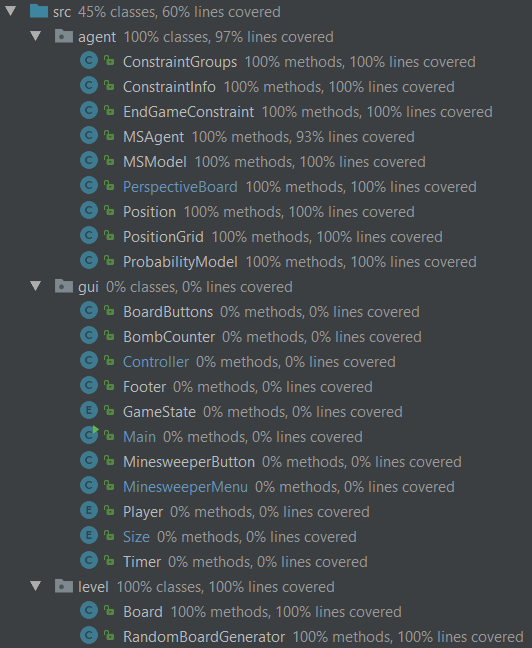
\includegraphics[scale=0.95]{test.png}
\end{center}
\caption{Code coverage}
\label{fig:cov}
\end{figure}
Highlights of tests include:
\begin{itemize}
\item Simulating several thousands of games, showing statistics.
\item Comparing probabilities calculated by hand vs one with the constraint model.
\item Testing wins on levels that don't need guessing by manually choosing first move.
\item Internal updating and data structures.
\item Contradicting assumption given specific game scenarios.
\item Division of constraint groups.
\end{itemize}

\section{Source code}
A GitHub repository can be found on my \href{https://github.com/JonSteinn}{GitHub page} and \href{https://github.com/JonSteinn/Minesweeper/archive/master.zip}{here} is a direct download link. This includes the Choco library.
\section{Demo}
\href{https://www.youtube.com/watch?v=ocDPL8nYT2o}{Here} is a video demo of the GUI and the solver in action on youtube.


\newpage
\begin{thebibliography}{2}
\bibitem{wiki} Minesweeper, Wikipedia, https://en.wikipedia.org/wiki/Minesweeper\_(video\_game), 6.3.2017.
\bibitem{npc} Kaye, Richard, \emph{Minesweeper is NP-complete}, Mathematical Intelligencer, vol 22, number 2, pp9-15, 2000.
\end{thebibliography}

\end{document}





















































